\addcontentsline{toc}{subsection}{Imagens}
\subsection*{Imagens}

\begin{figure}[ht]
	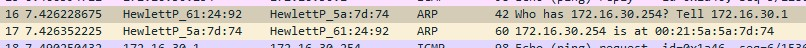
\includegraphics[width=\linewidth]{figure1}                                                      
    \caption{Pacotes ARP}
    \label{fig:fig1}
\end{figure}

\begin{figure}[ht]
	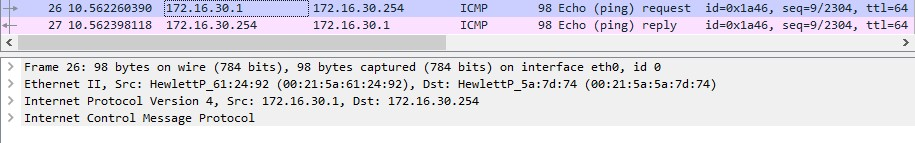
\includegraphics[width=\linewidth]{figure2}                                                      
    \caption{Pacote de Pedido}
    \label{fig:fig2}
\end{figure}

\begin{figure}[ht]
	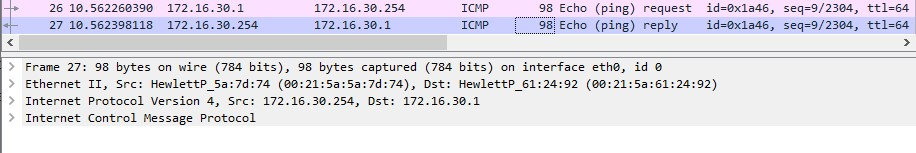
\includegraphics[width=\linewidth]{figure3}                                                      
    \caption{Pacote de Resposta}
    \label{fig:fig3}
\end{figure}

\begin{figure}[ht]
	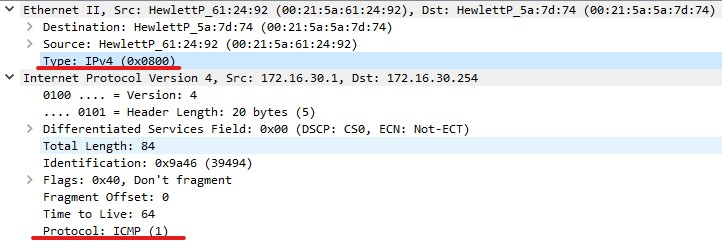
\includegraphics[width=\linewidth]{figure4}                                                      
    \caption{Campo Type Pacote ICMP}
    \label{fig:fig4}
\end{figure}

\begin{figure}[ht]
	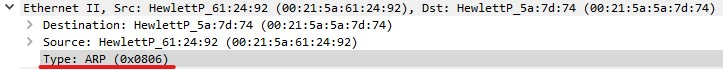
\includegraphics[width=\linewidth]{figure5}                                                      
    \caption{Campo Type Pacote ARP}
    \label{fig:fig5}
\end{figure}

\begin{figure}[ht]
	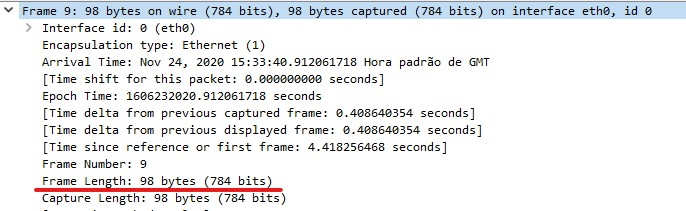
\includegraphics[width=\linewidth]{figure6}                                                      
    \caption{Tamanho de uma trama Recetora}
    \label{fig:fig6}
\end{figure}

\begin{figure}[ht]
	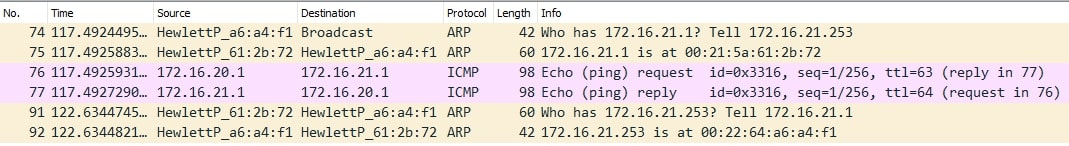
\includegraphics[width=\linewidth]{figure7}                                                      
    \caption{Pacotes ARP carta eth1 tux4}
    \label{fig:fig7}
\end{figure}

\begin{figure}[ht]
	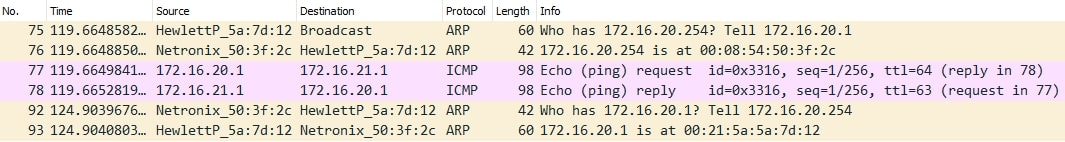
\includegraphics[width=\linewidth]{figure8}                                                      
    \caption{Pacotes ARP carta eth0 tux4}
    \label{fig:fig8}
\end{figure}

\begin{figure}[ht]
	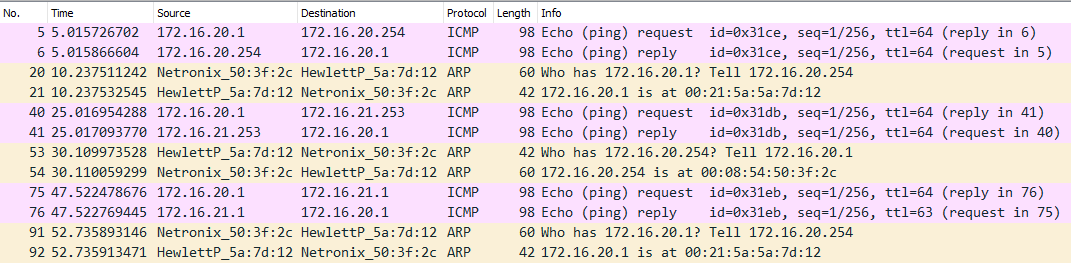
\includegraphics[width=\linewidth]{figure9}                                                      
    \caption{Pacotes ICMP com rotas definidas}
    \label{fig:fig9}
\end{figure}


